\documentclass{beamer}
\mode<presentation>
\usetheme{CambridgeUS}
\usecolortheme{beaver}
\setbeamertemplate{caption}[numbered]

\usepackage[english]{babel}
\usepackage{graphicx}
\usepackage{subfigure}
\usepackage{url}
\usepackage[backend=bibtex, style=verbose]{biblatex}
\usepackage{multicol}
\bibliography{bibliography.bib}
\usepackage[noend]{algorithm,algpseudocode}
\usepackage[justification=centering]{caption}


\title[LSTM: A Search Space Odysseys]{LSTM: A Search Space Odysseys}
\author[Mu\c sat Bogdan-Adrian]{Mu\c sat Bogdan-Adrian}
\date{February 2017}

\beamertemplatenavigationsymbolsempty
\graphicspath{{./images/}}

\begin{document}

\frame{\titlepage}

\begin{frame}
\frametitle{Recurrent Neural Networks - RNNs}
\center
\begin{itemize}
	\item Used to deal with sequential data, where there is a temporal dependence from a time instance to another
	\item Mathematically, they model a conditional distribution of the form \(P(x_t \lvert x_{t-1},..., x_2, x_1) \), where \(x_t\) is the current input at time \(t\)
	\item The output of a vanilla RNN cell at each time step is computed using the current input \(x_t\) and also the previous cell state \(h_{t-1}\)\footnote{Meant to encompass a summary of the past information} as:
	\[
		y_t = tanh(Ux_t + Wh_{t-1} + b),
	\]
	where \(U \in R^{M \times N}\), \(W \in R^{N \times N}\) are the shared parameter matrices for the RNN cells and \(b \in R^N\) is the bias
\end{itemize}
\end{frame}

\begin{frame}
\frametitle{Recurrent Neural Networks Unrolled}
\begin{figure}
        {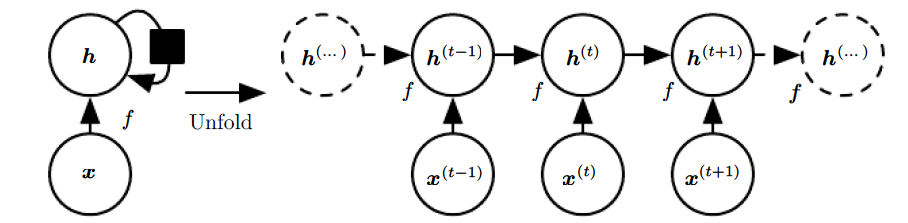
\includegraphics[width=0.65\textwidth]{rnn_unrolled.png}}
        \caption{RNN unrolled \footcite{Goodfellow-et-al-2016}}
    \end{figure}
\end{frame}

\begin{frame}
\frametitle{Backpropagation Through Time}
\begin{figure}
        {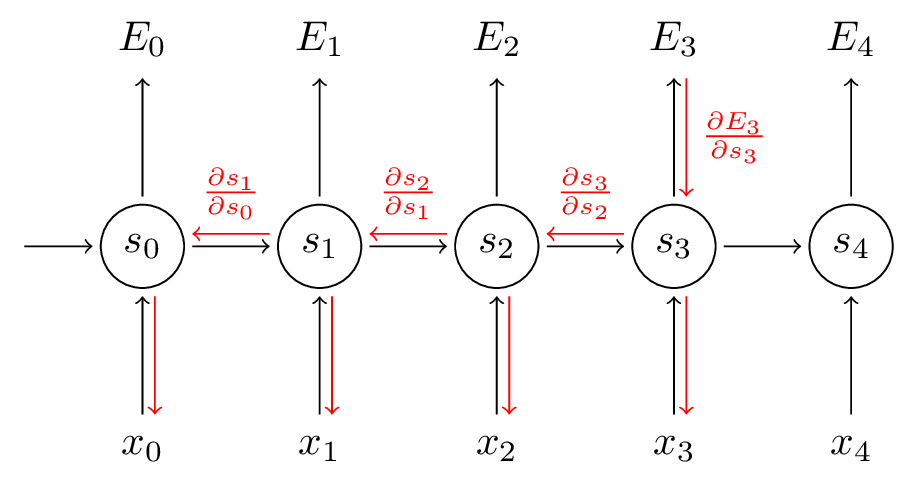
\includegraphics[width=0.9\textwidth]{bptt.png}}
        \caption{Backpropagation through time}
    \end{figure}
\end{frame}

\begin{frame}
\frametitle{Vanishing/Exploding Gradient}
\begin{itemize}
	\item The main algorithm for learning the weights of an RNN is called Backpropagation Through Time (BPTT)
	\item When computing the gradients with respect to the weights of the network, \(W\) depends on a recurrent connection from a previous timestep and so the partial derivative w.r.t. \(W\) becomes:
	\[
		\frac{\partial L^{(t)}}{\partial W} = \sum_{k=0}^{t} \frac{\partial L^{(t)}}{\partial o^{(t)}} \frac{\partial o^{(t)}}{\partial h^{(t)}} \bigg( \prod_{j=k+1}^t \frac{\partial h^{(j)}}{\partial h^{(j-1)}} \bigg) \frac{\partial h^{(k)}}{\partial W},
	\]
	where \(L^{(t)}\) is the error and \(o^{(t)}\) is the predicted value at the \(t^{th}\) output step
	\item If the number of timesteps is big, the product from the formula above will either diminish to \(0\) or explode to \(\infty\), thus prohibiting the learning process further on
\end{itemize}
\end{frame}

\begin{frame}
\frametitle{Long Short-Term Memory - LSTM}
\begin{itemize}
	\item LSTM\footcite{lstm} solves the problem of vanishing/exploding gradients
	\item The LSTM architecture is a memory cell, which can maintain its state over time, and nonlinear gating units, which regulate the information flow into and out of the cell
	\item Further experiments have proven that no other variants that differ from the vanilla LSTM by adding, removing or modifying exactly one aspect can obtain a much better performance \footcite{DBLP:journals/corr/GreffSKSS15}
\end{itemize}
\end{frame}

\begin{frame}
\frametitle{LSTM Cell}
\begin{figure}
        {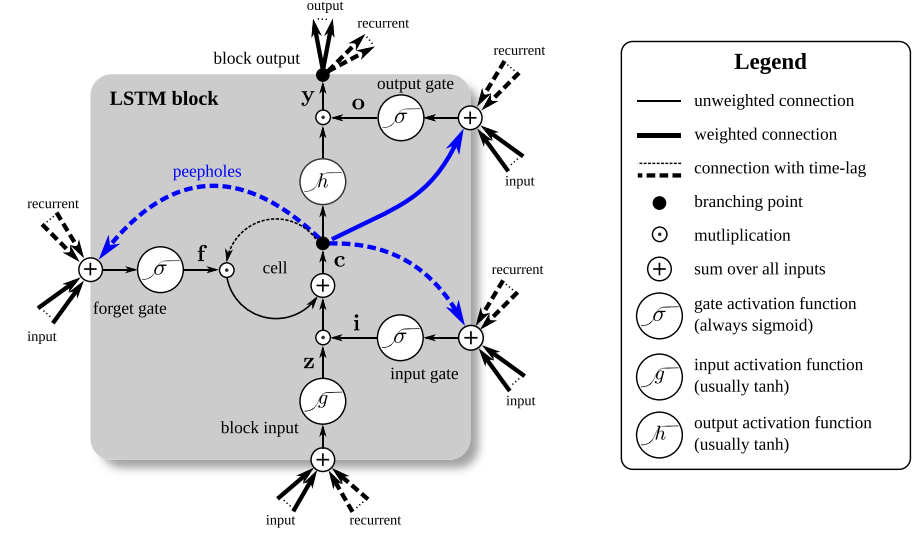
\includegraphics[width=0.9\textwidth]{lstm_cell.png}}
        \caption{LSTM cell} 
    \end{figure}
\end{frame}

\begin{frame}
\frametitle{LSTM Cell Computation}
\begin{itemize}
	\item The formulas for a vanilla LSTM layer forward pass can be written as:
	\begin{align*}
		&\bar{z}^t = W_z x^t + R_z y^{t-1} + b_z& \\
		&z^t = g(\bar{z}^t)& \text{block input} \\
		&\bar{i}^t = W_i x^t + R_i y^{t-1} + p_i \odot c^{t-1} + b_i& \\
		&i^t = \sigma (\bar{i}^t)& \text{input gate} \\
		&\bar{f}^t = W_f x^t + R_f y^{t-1} + p_f \odot c^{t-1} + b_f& \\
		&f^t = \sigma (\bar{f}^t)& \text{forget gate} \\
		&c^t = z^t \odot i^t + c^{t-1} \odot f^t& \text{cell} \\
		&\bar{o}^t = W_o x^t + R_o y^{t-1} + p_o \odot c^{t-1} + b_o& \\
		&o^t = \sigma (\bar{o}^t)& \text{output gate} \\
		&y^t = h(c^t) \odot o^t& \text{block output}
	\end{align*}
\end{itemize}
\end{frame}

\begin{frame}
\frametitle{LSTM Gates}
\begin{itemize}
	\item Each gate is computed in terms of the current input, the previous output, a peephole connection to the previous cell state and a bias
	\item \(i^t\), \(f^t\) and \(o^t\) are called the input, forget and output gates and their role is to determine how much information flows from previous and current timesteps. This effect is achieved by squashing the gates through a sigmoid function. Then an element wise multiplication is performed such that the input gate determines how much of the current information is used, the forget gate deals with the information flow from the previous cell state and finally, the output gate specifies how much information to send to the output \(y\)
	\item The peephole connections were added such that the network can learn precise timings easier \footcite{Gers:2003:LPT:944919.944925}
\end{itemize}
\end{frame}

\begin{frame}
\frametitle{Evaluation Setup}
\begin{itemize}
	\item The vanilla LSTM is used as a baseline and evaluated together with eight of its variants
	\item Random search was used to obtain good-performing hyperparameters
	\item Three datasets were used to evaluate the performance
	\begin{itemize}
		\item The TIMIT Speech corpus
		\item The IAM Online Handwriting Database
		\item JSB Chorales
	\end{itemize}
	\item The interaction between hyperparameters was observed using the fANOVA framework\footcite{HutHooLey14}
\end{itemize}
\end{frame}

\begin{frame}
\frametitle{LSTM Variants}
\begin{itemize}
	\item \textbf{NIG:} No Input Gate: \(i^t = 1\)
	\item \textbf{NFG:} No Forget Gate: \(f^t = 1\)
	\item \textbf{NOG:} No Output Gate: \(o^t = 1\)
	\item \textbf{NIAF:} No Input Activation Function: \(g(x) = x\)
	\item \textbf{NOAF:} No Output Activation Function: \(h(x) = x\)
	\item \textbf{CIFG:} Coupled Input and Forget Gate: \(f^t = 1 - i^t\)
	\item \textbf{NP:} No Peepholes:
	\begin{align*}
		&\bar{i}^t = W_i x^t + R_i y^{t-1} + b_i& \\
		&\bar{f}^t = W_f x^t + R_f y^{t-1} + b_f& \\
		&\bar{o}^t = W_o x^t + R_o y^{t-1} + b_o& \\
	\end{align*}
\end{itemize}
\end{frame}

\begin{frame}
\frametitle{LSTM Variants}
\begin{itemize}
	\item \textbf{FGR:} Full Gate Recurrence:
	\begin{align*}
		\bar{i}^t = &W_i x^t + R_i y^{t-1} + p_i \odot c^{t-1} + b_i \\
					&+ R_{ii} i^{t-1} + R_{fi} f^{t-1} + R_{oi} o^{t-1} \\
		\bar{f}^t = &W_f x^t + R_f y^{t-1} + p_f \odot c^{t-1} + b_f \\
					&+ R_{if} i^{t-1} + R_{ff} f^{t-1} + R_{of} o^{t-1} \\
		\bar{o}^t = &W_o x^t + R_o y^{t-1} + p_o \odot c^{t-1} + b_o \\
					&+ R_{io} i^{t-1} + R_{fo} f^{t-1} + R_{oo} o^{t-1}
	\end{align*}
	\item The CIFG variant is also known as Gated Recurrent Unit (GRU) \footcite{DBLP:journals/corr/ChoMGBSB14}
	\item The FGR variant adds recurrent connections between all the gates, thus significantly increasing the number of parameters
\end{itemize}
\end{frame}

\begin{frame}
\frametitle{Results}
\begin{itemize}
	\item Figure 3 represents the test set performance for all 200 trials (top) and for the best 10\% (bottom) trials (according to the validation set) for each data set and variant.
Boxes: range between the 25th and 75th percentiles of the data. Whiskers: whole range. Red dot: mean. Red line: median of the data. Thick blue lines: boxes
of variants that differ significantly from the vanilla LSTM. Gray histogram in the background: average number of parameters for the top 10\% performers of
every variant.
\end{itemize}
\end{frame}

\begin{frame}
\frametitle{Results}
\begin{figure}
        {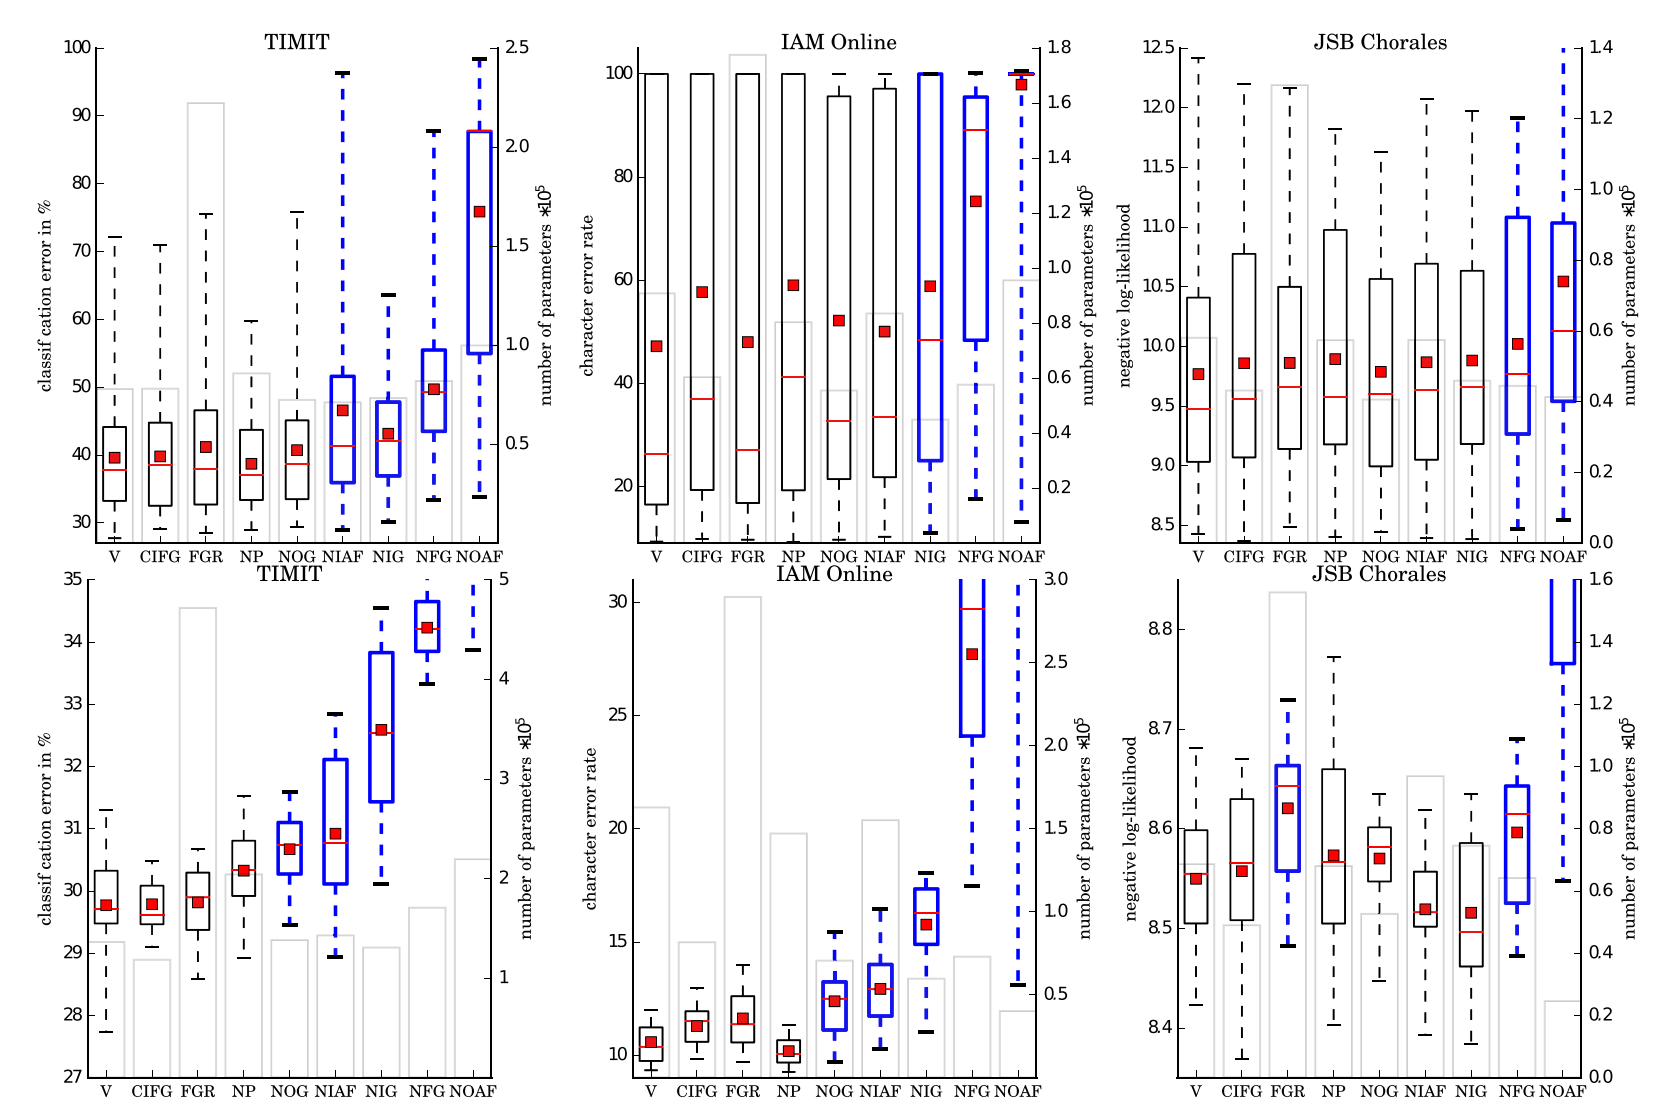
\includegraphics[width=0.8\textwidth]{results.png}}
        \caption{Box plots for the test performance}
    \end{figure}
\end{frame}

\begin{frame}
\frametitle{Observations}
\begin{itemize}
	\item Removing the output activation function (NOAF) or the forget gate (NFG) significantly hurt performance on all three data sets
	\item Input and forget gate coupling (CIFG) did not significantly change the mean performance on any of the data sets
	\item Removing the peephole connections (NP) also did not lead to significant changes
	\item Adding FGR does not significantly change performance, but increases the number of parameters
	\item For supervised learning on continuous real-valued data the input gate, output gate, and input activation function are crucial
\end{itemize}
\end{frame}

\begin{frame}
\frametitle{Impact of Hyperparameters}
\begin{itemize}
	\item The fANOVA framework for assessing hyperparameters importance is based on the observation that marginalizing over dimensions can be done efficiently in regression trees. This allows predicting the marginal error for one hyperparameter while averaging over all the others
	\item The hyperparameter space is sampled at random
	\item The learning rate is determined as being the most important hyperparameter. A practical advice would be to tune it on a small network and then usee it to train a large one
	\item The hidden layer size is the second in order of importance. Larger networks perform better, but with diminishing returns.
	\item The additive Gaussian noise on the inputs almost always hurt performance and slightly increases training times
	\item Momentum affects neither performance nor training time in any significant way
\end{itemize}
\end{frame}

\begin{frame}
\frametitle{Analysis of Variance}
\begin{figure}
        {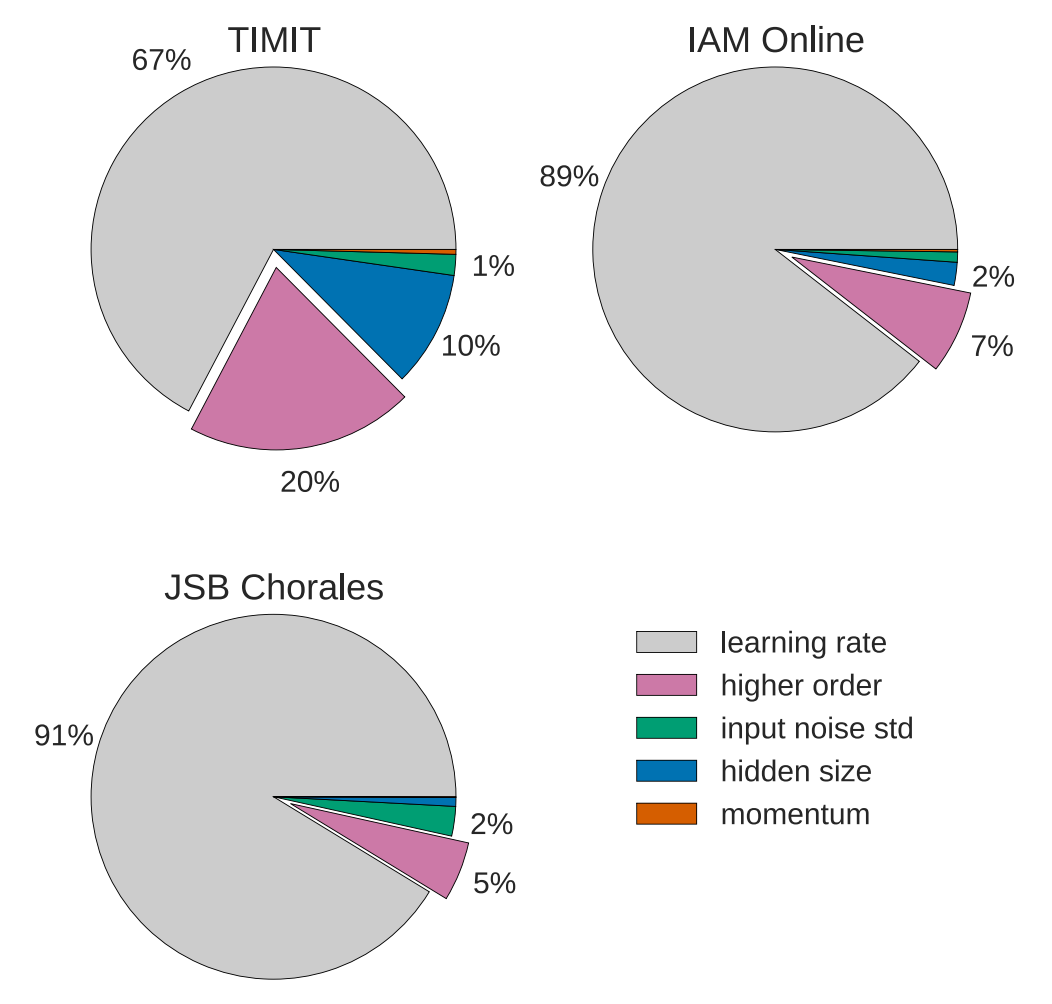
\includegraphics[width=0.5\textwidth]{variance_analysis.png}}
        \caption{Pie charts showing which fraction of variance of the test set performance can be attributed to each of the hyperparameters}
    \end{figure}
\end{frame}

\begin{frame}
\frametitle{Interaction of Hyperparameters}
\begin{figure}	
        {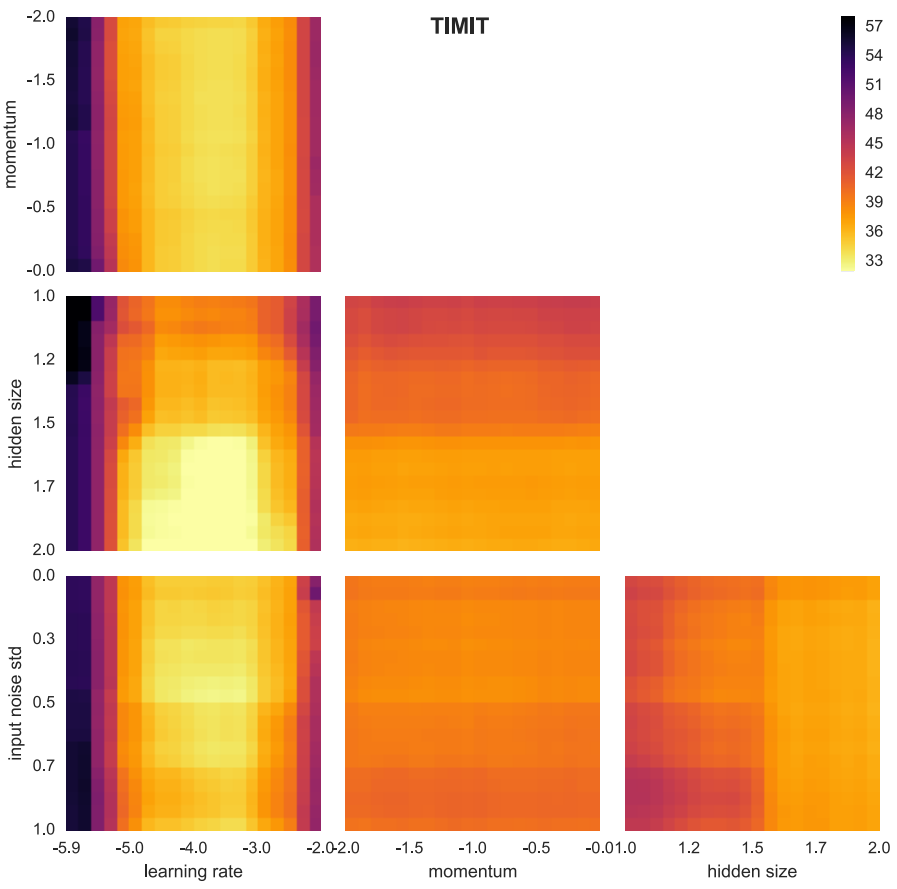
\includegraphics[width=0.55\textwidth]{timit_variance.png}}
        \caption{Hyperparameter interaction on TIMIT}
    \end{figure}
\end{frame}

\begin{frame}
\frametitle{Interaction of Hyperparameters}
\begin{figure}
        {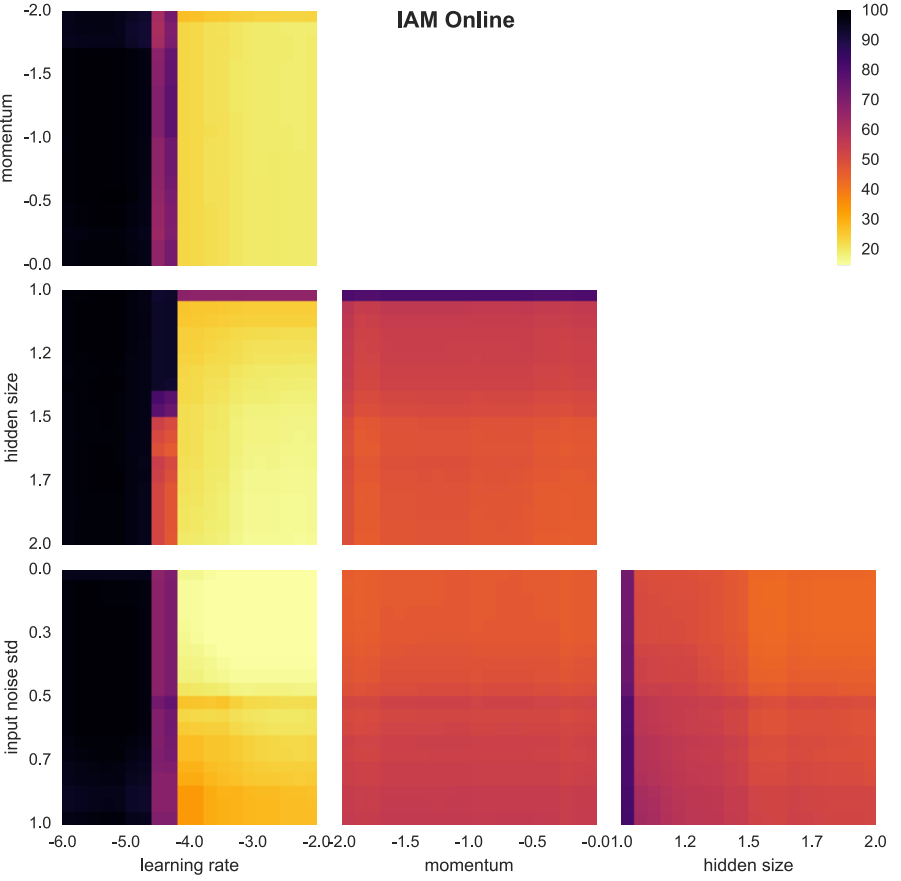
\includegraphics[width=0.55\textwidth]{iam_variance.png}}
        \caption{Hyperparameter interaction on IAM Online}
    \end{figure}
\end{frame}

\begin{frame}
\frametitle{Interaction of Hyperparameters}
\begin{figure}
        {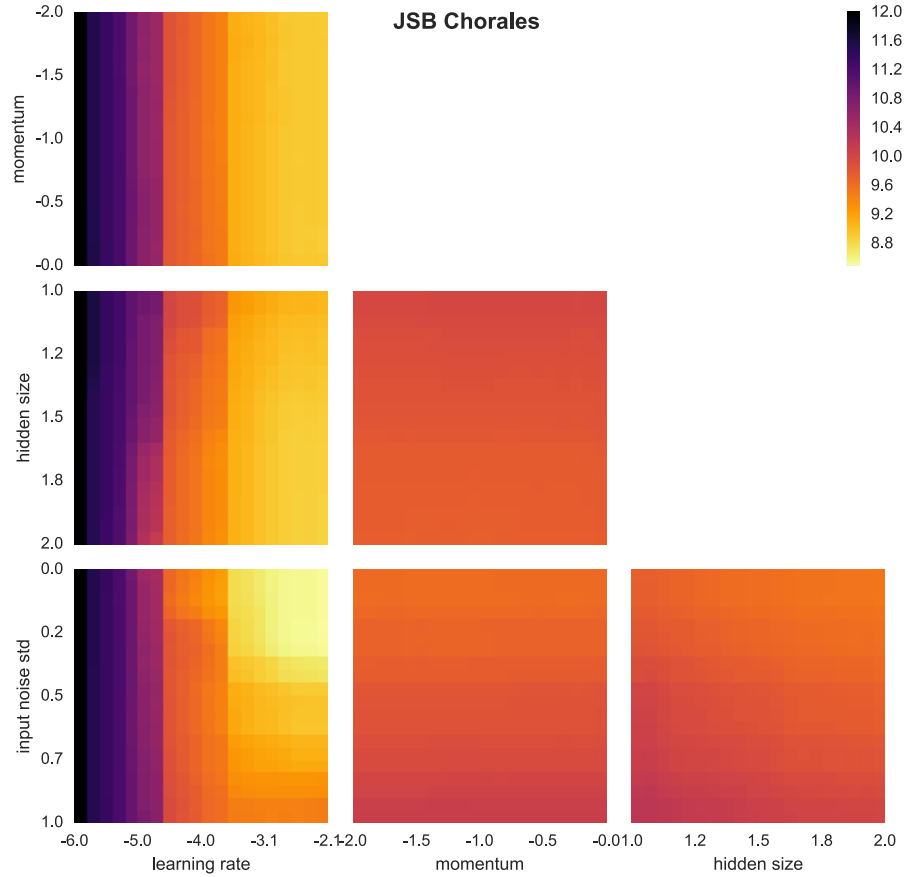
\includegraphics[width=0.55\textwidth]{jsb_variance.png}}
        \caption{Hyperparameter interaction on JSB Chorales}
    \end{figure}
\end{frame}

\begin{frame}
\frametitle{Conclusions}
\begin{itemize}
	\item Vanilla LSTM performs reasonably well on a various data sets, none of the eight investigated modifications significantly improving the performance
	\item Simpler LSTM variants like CIFG and NP might be attractive because of the reduction in the number of parameters
	\item The forget gate and the output activation function are the most critical components of the LSTM block
	\item The learning rate is the most important hyperparameter, followed by the network size
	\item The analysis of hyperparameters interaction revealed no apparent structure, meaning that they can be treated as approximately independent
\end{itemize}
\end{frame}

\begin{frame}
\frametitle{Technical Slides - Vanishing/Exploding Gradients Derivations}
	\begin{align*}
		\frac{\partial L}{\partial W} &= \sum_{t=0}^{S} \frac{\partial L^{(t)}}{\partial W}&\\
		\frac{\partial L^{(t)}}{\partial W} &= \sum_{k=0}^{t} \frac{\partial L^{(t)}}{\partial 		o^{(t)}} \frac{\partial o^{(t)}}{\partial h^{(t)}} \frac{\partial h^{(t)}}{\partial h^{(k)}} \frac{\partial h^{(k)}}{\partial W}&\\
		\frac{\partial h^{(t)}}{\partial h^{(k)}} &= \prod_{i=k+1}^{t} \frac{\partial h^{(i)}}{\partial h^{(i-1)}}&\\
		\frac{\partial L^{(t)}}{\partial W} &= \sum_{k=0}^{t} \frac{\partial L^{(t)}}{\partial o^{(t)}} \frac{\partial o^{(t)}}{\partial h^{(t)}} \bigg( \prod_{j=k+1}^t \frac{\partial h^{(j)}}{\partial h^{(j-1)}} \bigg) \frac{\partial h^{(k)}}{\partial W}&
	\end{align*}
\end{frame}

\end{document}